% !TeX encoding = UTF-8

\chapter{FUNDAMENTAÇÃO TEÓRICA}\label{ch:fundaments-teorico}
A mineração de dados é um assunto totalmente interdisciplinar, ...

%%
% KDD
\section{DESCOBERTA DE CONHECIMENTO EM BASE DE DADOS E \textit{DATA MINING}}\label{sec:kdd}
Muitas pessoas tratam a mineração de dados ... O processo de KDD é demonstrado através da  \autoref{kdd-fig} e, posteriormente, listada como uma sequência interativa e iterativa dos seguintes passos:

\begin{figure}[h]
	\centering
	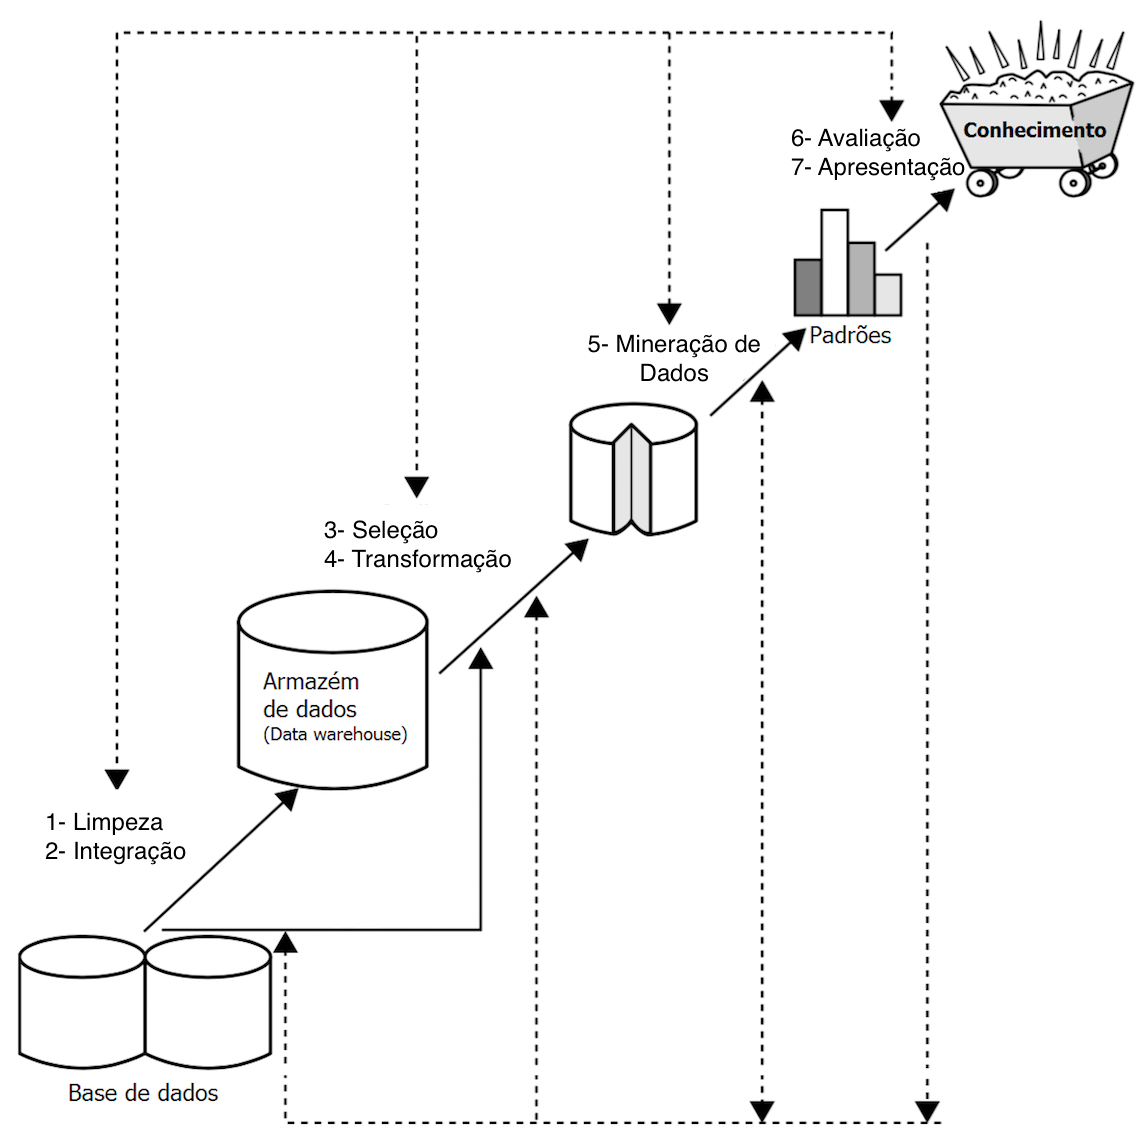
\includegraphics[width=.5\textwidth]{kdd2}
	\caption{Etapas do processo de KDD}
	\fonte{Adaptado de \citeonline{han}}
	\label{kdd-fig}
\end{figure}

\begin{enumerate}
	\item \textit{Data cleaning} (Limpeza de dados);
	\item \textit{Data integration} (Integração de dados);
	\item \textit{Data selection} (Seleção de dados);
	\item \textit{Data transformation} (Transformação de dados);
	\item \textit{Data mining} (Mineração de dados);
	\item \textit{Pattern evaluation} (Avaliação de padrões);
	\item \textit{Knowledge presentation} (Apresentação de conhecimento).
\end{enumerate}

É importante notar que algum dos processos acontecem na mesma etapa: Limpeza e integração; Seleção e transformação; Avaliação e apresentação.

De acordo com \apudonline{brachman}{fayyad2}, as etapas são interativas ....















